\notechapter{N-20260318}{Matrix Computation III: Canonical Forms, Localization, and Iteration}

\section{Why canonical forms matter}

Canonical forms explain what a matrix cannot hide under a change of basis.  For computation they answer: how do powers behave, where can eigenvalues be, and which direction dominates an iteration?

\section{Polynomial matrices}

A \(\lambda\)-matrix is a matrix whose entries lie in \(\mathbb C[\lambda]\).  Its rank is the largest order of a minor that is not the zero polynomial.  A square \(\lambda\)-matrix is nonsingular if its determinant is not the zero polynomial.

The elementary operations are row or column exchange, multiplication of a row or column by a nonzero constant, and adding \(\varphi(\lambda)\) times one row or column to another.

\section{Smith normal form}

Every rank \(r\) polynomial matrix is equivalent to
\[
  \operatorname{diag}(d_1(\lambda),\ldots,d_r(\lambda),0,\ldots,0),
\]
where each \(d_i\) is monic and
\[
  d_1\mid d_2\mid\cdots\mid d_r.
\]
This is the Smith normal form.

Let \(D_k(\lambda)\) be the monic greatest common divisor of all nonzero \(k\)-minors.  The invariant factors are
\[
  d_1=D_1,\qquad d_k=\frac{D_k}{D_{k-1}}.
\]
Factoring the nonconstant invariant factors gives elementary divisors.

\section{Jordan data from elementary divisors}

For \(A\in\mathbb C^{n\times n}\), apply Smith form to
\[
  \lambda I-A.
\]
An elementary divisor
\[
  (\lambda-\lambda_0)^s
\]
corresponds to a Jordan block of size \(s\) for eigenvalue \(\lambda_0\).

Thus Smith form is an algebraic route to Jordan structure.

\section{Jordan chains}

A Jordan block is
\[
  J_s(\lambda)=
  \begin{bmatrix}
  \lambda&1&&0\\
  &\lambda&\ddots&\\
  &&\ddots&1\\
  0&&&\lambda
  \end{bmatrix}.
\]
If \(A=PJP^{-1}\), the columns in one Jordan chain satisfy
\[
  Ap_1=\lambda p_1,\qquad
  Ap_i=\lambda p_i+p_{i-1}.
\]
The later vectors are generalized eigenvectors.

\section{Computing powers}

If \(J=\lambda I+N\) with \(N^s=0\), then
\[
  J^k=\sum_{j=0}^{s-1}\binom{k}{j}\lambda^{k-j}N^j.
\]
For \(A=PJP^{-1}\),
\[
  A^k=PJ^kP^{-1}.
\]
Jordan form explains polynomial factors in matrix powers.

\section{Gershgorin discs}

For \(A=(a_{ij})\), define
\[
  R_i=\sum_{j\ne i}|a_{ij}|.
\]
Every eigenvalue lies in
\[
  \bigcup_i \{z\in\mathbb C: |z-a_{ii}|\le R_i\}.
\]
Proof: choose \(i\) with \(|x_i|=\max_j|x_j|\) for an eigenvector \(x\).  From \(Ax=\lambda x\),
\[
  (\lambda-a_{ii})x_i=\sum_{j\ne i}a_{ij}x_j,
\]
so \(|\lambda-a_{ii}|\le R_i\).

\section{Gershgorin figure}

\begin{figure}[H]
\centering
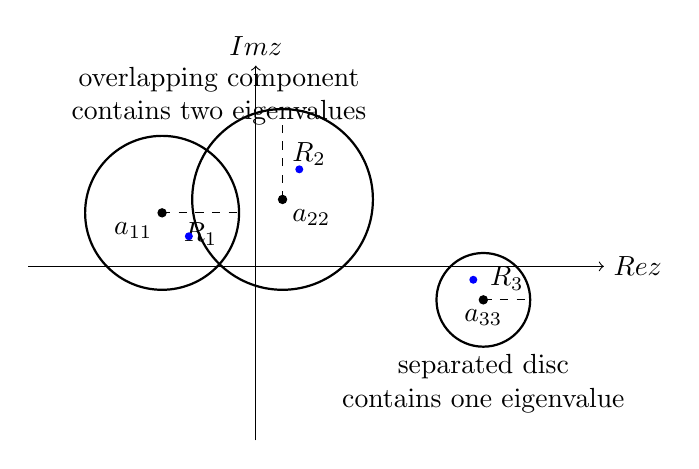
\begin{tikzpicture}[scale=0.85]
  \draw[->] (-3.4,0) -- (5.2,0) node[right] {$\operatorname{Re}z$};
  \draw[->] (0,-2.6) -- (0,3.0) node[above] {$\operatorname{Im}z$};
  \coordinate (c1) at (-1.4,0.8);
  \coordinate (c2) at (0.4,1.0);
  \coordinate (c3) at (3.4,-0.5);
  \draw[thick] (c1) circle (1.15);
  \draw[thick] (c2) circle (1.35);
  \draw[thick] (c3) circle (0.7);
  \fill (c1) circle (2pt) node[below left] {$a_{11}$};
  \fill (c2) circle (2pt) node[below right] {$a_{22}$};
  \fill (c3) circle (2pt) node[below] {$a_{33}$};
  \draw[dashed] (c1) -- ++(1.15,0) node[midway,below] {$R_1$};
  \draw[dashed] (c2) -- ++(0,1.35) node[midway,right] {$R_2$};
  \draw[dashed] (c3) -- ++(0.7,0) node[midway,above] {$R_3$};
  \node[align=center] at (-0.55,2.55) {overlapping component\\contains two eigenvalues};
  \node[align=center] at (3.4,-1.75) {separated disc\\contains one eigenvalue};
  \fill[blue] (-1.0,0.45) circle (1.7pt);
  \fill[blue] (0.65,1.45) circle (1.7pt);
  \fill[blue] (3.25,-0.2) circle (1.7pt);
\end{tikzpicture}
\caption{Gershgorin discs localize eigenvalues.  A separated component containing one disc contains exactly one eigenvalue.}
\end{figure}

\section{Separated components and scaling}

If a connected component of the union of Gershgorin discs consists of exactly \(m\) discs and is separated from the others, then it contains exactly \(m\) eigenvalues.

Column Gershgorin discs can be obtained by applying the theorem to \(A^T\).  Diagonal similarity
\[
  D^{-1}AD
\]
does not change eigenvalues but changes radii, since
\[
  (D^{-1}AD)_{ij}=d_i^{-1}a_{ij}d_j.
\]
This is a practical way to improve localization.

\section{Power iteration}

If
\[
  |\lambda_1|>|\lambda_2|\ge\cdots,
\]
and the initial vector has a nonzero component in the dominant eigenvector direction, then
\[
  u_{k+1}=\frac{Au_k}{\|Au_k\|}
\]
converges toward the dominant eigenvector direction.  The convergence rate is governed by
\[
  \left|\frac{\lambda_2}{\lambda_1}\right|.
\]

\section{Inverse and shifted inverse iteration}

Inverse iteration applies power iteration to \(A^{-1}\), so it finds eigenvalues of small modulus.  Shifted inverse iteration applies inverse iteration to
\[
  A-pI.
\]
Eigenvalues of \((A-pI)^{-1}\) are
\[
  \frac1{\lambda_j-p}.
\]
Thus the eigenvalue closest to \(p\) becomes dominant.

\section{Numerical traps}

Shifted inverse iteration requires solving systems with \(A-pI\), which may be nearly singular.  This is why the method can be powerful and unstable at the same time.  Pivoting and residual checks are essential.

Gershgorin discs are cheap localization, not exact computation.  Overlap does not mean eigenvalues are evenly spread through the overlap.

\section{ML-facing interpretation}

Power iteration appears in PageRank, spectral normalization, graph propagation, and monitoring dominant eigenvalue behavior.  State-space and recurrent models depend on polynomial and spectral structure: the minimal polynomial, Jordan blocks, and spectral radius all describe memory and long-run dynamics.

\section{Checklist}

\[
\begin{array}{c|c}
\text{Smith form} & \text{invariant factors}\\
\text{Jordan form} & \text{eigenvalue chains}\\
\text{Gershgorin} & \text{cheap eigenvalue regions}\\
\text{power iteration} & \text{dominant eigenvalue}\\
\text{shifted inverse iteration} & \text{eigenvalue near target}
\end{array}
\]
